\documentclass{ximera}

\title{Multivariable Optimization: Gradient Descent Applet}
\author{Zack Reed}

\begin{document}
\begin{abstract}
In this activity we engage with an applet that dynamically explores the use of gradient descent to linearly fit a line to data.
\end{abstract}
\maketitle

\section*{The Main Goal: Approximating Data With a Line}

In this activity you can dynamically explore gradient descent and how it can be used to minimize the error created in some approximation process.

Here, the task is to define a line that as closely as possible runs through a set of data points. The line will be defined by two parameters: the slope $m$ and the $y$-intercept $b$. The error in the approximation is defined as the sum of the squared vertical distances from each data point to the line.

For instance, for the following 20 data points found in the graph below:

%a tikz image of data points
\begin{center}
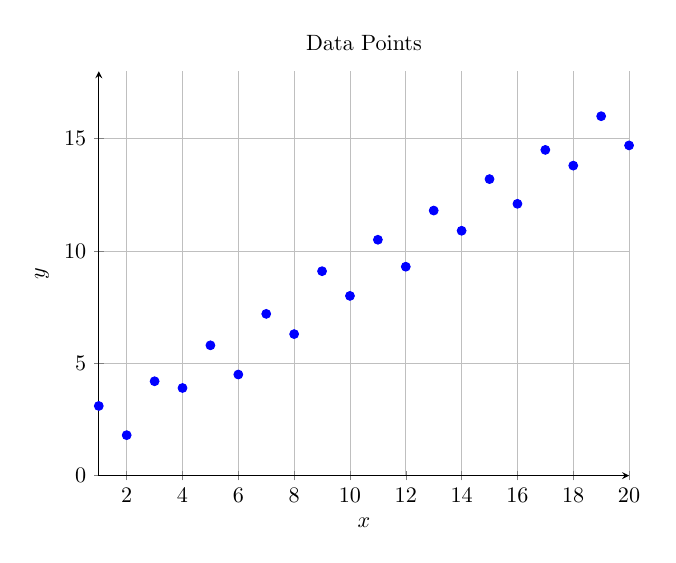
\begin{tikzpicture}[scale=0.8]
    \begin{axis}[
        axis lines = left,
        xlabel = $x$,
        ylabel = {$y$},
        title = {Data Points},
        width=10cm,
        height=8cm,
        grid=major,
        ymin=0, ymax=18,
    ]
    \addplot[only marks, mark=*, blue] coordinates {
        (1,3.1) (2,1.8) (3,4.2) (4,3.9) (5,5.8)
        (6,4.5) (7,7.2) (8,6.3) (9,9.1) (10,8.0)
        (11,10.5) (12,9.3) (13,11.8) (14,10.9) (15,13.2)
        (16,12.1) (17,14.5) (18,13.8) (19,16.0) (20,14.7)
    };
    \end{axis}
\end{tikzpicture}
\end{center}

we want to find the line $y = mx + b$ that minimizes the error between the height of the line and the height of each data point.

%a tikz image of data points and a line and the error lines
\begin{center}
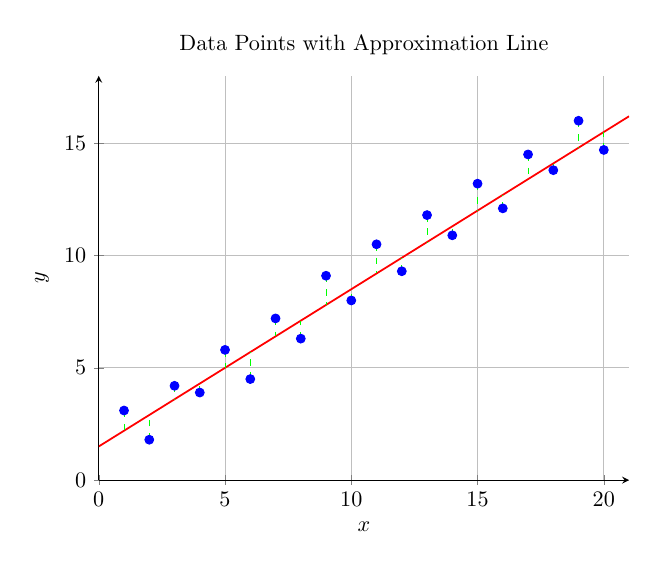
\begin{tikzpicture}[scale=0.8]
    \begin{axis}[
        axis lines = left,
        xlabel = $x$,
        ylabel = {$y$},
        title = {Data Points with Approximation Line},
        width=10cm,
        height=8cm,
        grid=major,
        ymin=0, ymax=18,
    ]
    \addplot[only marks, mark=*, blue] coordinates {
        (1,3.1) (2,1.8) (3,4.2) (4,3.9) (5,5.8)
        (6,4.5) (7,7.2) (8,6.3) (9,9.1) (10,8.0)
        (11,10.5) (12,9.3) (13,11.8) (14,10.9) (15,13.2)
        (16,12.1) (17,14.5) (18,13.8) (19,16.0) (20,14.7)
    };
    \addplot[red, thick, domain=0:21] {0.7*x + 1.5}; % Example line
    \addplot[green, dashed] coordinates {(1,3.1) (1,2.2)};
    \addplot[green, dashed] coordinates {(2,1.8) (2,2.9)};
    \addplot[green, dashed] coordinates {(3,4.2) (3,3.6)};
    \addplot[green, dashed] coordinates {(4,3.9) (4,4.3)};
    \addplot[green, dashed] coordinates {(5,5.8) (5,5.0)};
    \addplot[green, dashed] coordinates {(6,4.5) (6,5.7)};
    \addplot[green, dashed] coordinates {(7,7.2) (7,6.4)};
    \addplot[green, dashed] coordinates {(8,6.3) (8,7.1)};
    \addplot[green, dashed] coordinates {(9,9.1) (9,7.8)};
    \addplot[green, dashed] coordinates {(10,8.0) (10,8.5)};
    \addplot[green, dashed] coordinates {(11,10.5) (11,9.2)};
    \addplot[green, dashed] coordinates {(12,9.3) (12,9.9)};
    \addplot[green, dashed] coordinates {(13,11.8) (13,10.6)};
    \addplot[green, dashed] coordinates {(14,10.9) (14,11.3)};
    \addplot[green, dashed] coordinates {(15,13.2) (15,12.0)};
    \addplot[green, dashed] coordinates {(16,12.1) (16,12.7)};
    \addplot[green, dashed] coordinates {(17,14.5) (17,13.4)};
    \addplot[green, dashed] coordinates {(18,13.8) (18,14.1)};
    \addplot[green, dashed] coordinates {(19,16.0) (19,14.8)};
    \addplot[green, dashed] coordinates {(20,14.7) (20,15.5)};
    \end{axis}
\end{tikzpicture}
\end{center}

The green dashed lines represent the vertical distances from each data point to the line $y = 0.7x + 1.5$. While the details of how the error is calculated are not important for this activity, it is important to note that the error is a function of the parameters $m$ and $b$ that define the line. In this case, the mean squared error (MSE) for the line $y = 0.7x + 1.5$ is approximately $2.4$.

\section*{The Error Surface}

The error for any choice of slope $m$ and intercept $b$ creates a 3D surface, often called the "loss surface" or "error surface". For linear regression with squared error, this surface has a bowl shape with a single minimum point corresponding to the best-fit line.

\begin{center}
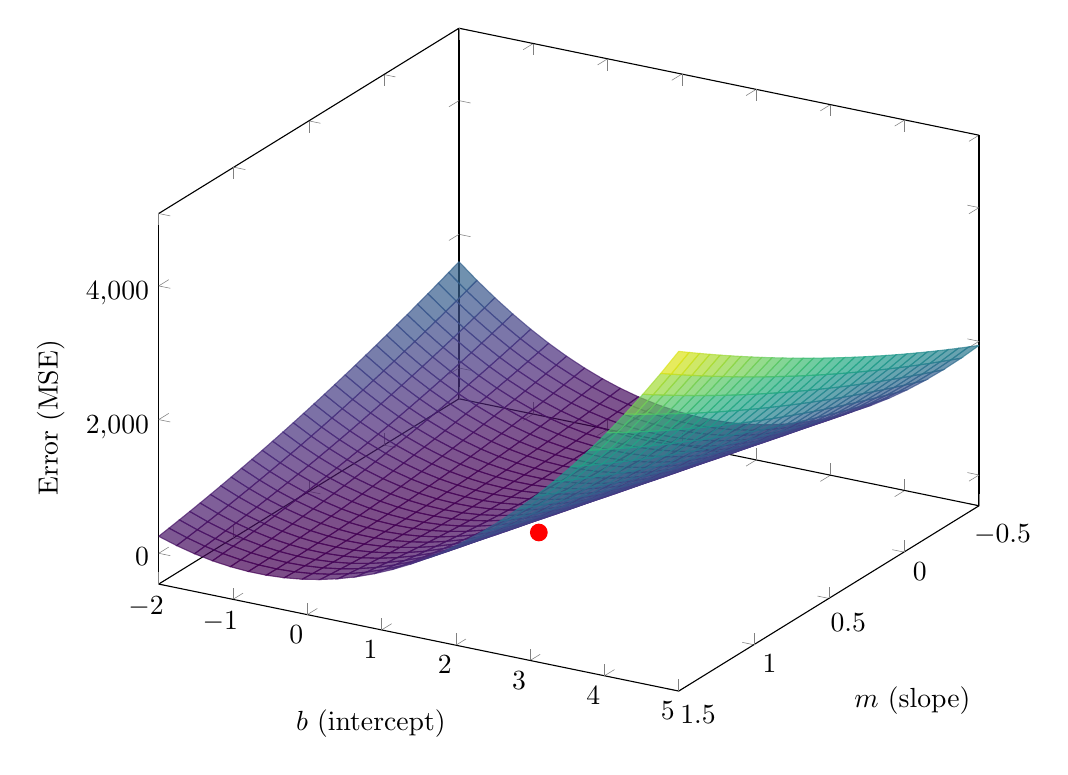
\begin{tikzpicture}
    \begin{axis}[
        view={120}{30},
        xlabel=$m$ (slope),
        ylabel=$b$ (intercept),
        zlabel={Error (MSE)},
        width=12cm,
        height=10cm,
        colormap/viridis,
    ]
    \addplot3[surf, opacity=0.7, shader=flat, domain=-0.5:1.5, domain y=-2:5, samples=30] 
        {((1*(x+y)-3.1)^2 + (2*(x+y)-1.8)^2 + (3*(x+y)-4.2)^2 + (4*(x+y)-3.9)^2 + 
          (5*(x+y)-5.8)^2 + (6*(x+y)-4.5)^2 + (7*(x+y)-7.2)^2 + (8*(x+y)-6.3)^2 + 
          (9*(x+y)-9.1)^2 + (10*(x+y)-8.0)^2 + (11*(x+y)-10.5)^2 + (12*(x+y)-9.3)^2 + 
          (13*(x+y)-11.8)^2 + (14*(x+y)-10.9)^2 + (15*(x+y)-13.2)^2 + (16*(x+y)-12.1)^2 + 
          (17*(x+y)-14.5)^2 + (18*(x+y)-13.8)^2 + (19*(x+y)-16.0)^2 + (20*(x+y)-14.7)^2)/20};
    \addplot3[only marks, mark=*, mark size=3, color=red] coordinates {(0.7, 1.5, 2.4)};
    \end{axis}
\end{tikzpicture}
\end{center}

The red point on the surface represents the error at $m=0.7$, $b=1.5$. Gradient descent is an algorithm that starts at some point on this surface and iteratively moves "downhill" (in the direction of steepest descent) to find the minimum.

\section*{Engaging with the Applet}

For technical reasons, the applet can be found at the following link: 
%link to https://zackreed.github.io/applets_for_learning_math/pages/gradient-descent-walkthrough.html
\begin{center}
\href{https://zackreed.github.io/applets_for_learning_math/pages/gradient-descent-walkthrough.html}{Gradient Descent Applet}
\end{center}

The page lets you adjust the possible slopes and $y$-intercepts of the line by dragging a point in $2D$-space, and then shows the possible lines that fit the data points. You can also view the error surface that shows the errors of all possible lines that might fit the data set. Finally, you can progressively use the gradient to to find the location on the error surface that has the lowest error, and thus find the line that best fits the data.

\end{document}
